\documentclass{article}
\usepackage[utf8]{inputenc}

\title{Obligatorisk innlevering 1}
\author{Sivert M. Skarning}
\date{Sept 2019}

\usepackage{natbib}
\usepackage{graphicx}

\begin{document}

\maketitle
\clearpage
\tableofcontents
\clearpage
\section{Oppgave 1}
\subsection{Oppgavebeskrivelse}
Etter hvert som medieselskapene har oppdaget at folk foretrekker tjenester som Netflix har stadig flere lansert egne strømmetjenester. Tjenestene tilbyr tilgang til medieinnhold til kunder som har aktive abonnement hos leverandøren. 

Du kan bruke hvilket verktøy du ønsker til å lage diagrammene, men vi anbefaler PlantUML (http://plantuml.com/ (Lenker til en ekstern side.)) (tekstbasert) eller draw.io (https://www.draw.io/ (Lenker til en ekstern side.)) (grafisk) som verktøy.

Lag use case-diagrammer som viser hva en kunde og en administrator kan gjøre i en slik tjeneste.
\subsection{Diagram}
\begin{figure}[h]
\centering
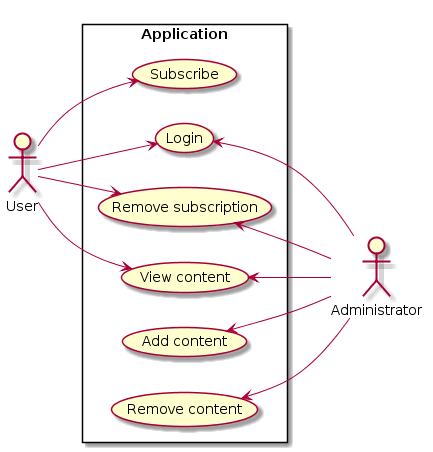
\includegraphics[scale=0.5]{images/oppgave1.png}
\caption{Usecase-diagram}
\label{fig:oppgave1.png}
\end{figure}

I dette systemet vil man ha en brukertype og en administratortype. Brukerne vil ha begrensede rettigheter. Administratoren vil ha utvidete rettigheter. Administrator vil ikke kunne ha muligheten til å legge til et abonnenment for en gitt bruker, dette er det kun brukeren selv som kan gjøre.

\section{Oppgave  2}
\subsection{Oppgavebeskrivelse}
Beskriv tre funksjonelle krav som stilles til systemet som en følge av use case-diagrammene. Bryt kravene opp i underkrav der det er nødvendig.
\subsection{Krav}
\paragraph{Funksjonelle krav}
\begin{itemize}
\item Lag abonnement
\item Legg til media
\item Fjern media
\item Vis valgt media
\end{itemize}

\paragraph{Ikke-funksjonelle krav}
\begin{itemize}
\item Må kunne håndtere flere brukere
\item Må kunne beskytte persondata
\end{itemize}

\section{Oppgave 3}
\subsection{Oppgavebeskrivelse}
Lag et sekvensdiagram som viser hvordan flyten mellom hvert lag i systemet kan være når en bruker ønsker å starte et abonnement. Anta at kunden betaler med et kredittkort. Bruk verb eller metodenavn som tekst over hver pil.

Tenk gjennom hvilke feilsituasjoner som kan oppstå og lag et sekvensdiagram som viser en slik situasjon.

\subsection{Sekvensdiagram for oprettelse av abonnement}
I figur \ref{fig:oppgave3} ser vi sekvensdiagrammet for en bruker som skal lage et abonnement. Diagrammet inneholder tre systemer, frontend, API og database.
\begin{figure}[h]
\centering
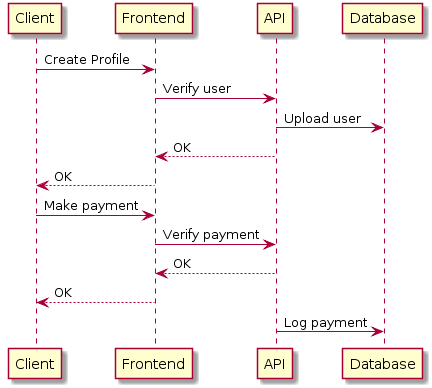
\includegraphics[scale=0.5]{images/oppgave3.png}
\caption{Sequence-diagram}
\label{fig:oppgave3}
\end{figure}

\subsection{Sekvensdiagram for feilhåndtering}
I et større system er det mange typer feil som kan intreffe. Feil som vi vet kan oppstå må håndteres.
\begin{itemize}
\item Intern nettverksfeil
\item Feil inndata
\item Feil fra eksterne systemer (som verifisering av kredittkort)
\end{itemize}

I dette eksemplet trekker jeg ut en feil ved inndata, brukeren har valgt et brukernavn som allerede finnes i systemet. Brukeren skal da få beskjed og muligheten til å kunne prøve med et annet brukernavn.

\begin{figure}[h]
\centering
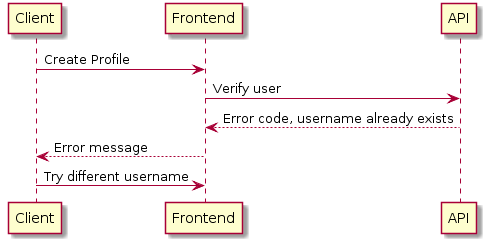
\includegraphics[scale=0.5]{images/oppgave3-2.png}
\caption{Sequencediagram for errorhandling}
\label{fig:oppgave3-2}
\end{figure}
\end{document}
